\chapter{Présentation générale}
\label{chap:presentationgenerale}

\section{Le menu principal}

La première interaction entre l'utilisateur consistera à choisir entre :

\begin{itemize}
    \item Jouer
    \item Tutoriel
    \begin{itemize}
    \item Manuel du jeu
    \item \sout{Didacticiel} (Une fois que le jeu sera totalement développé)
\end{itemize}
    \item Réglages
    \item Informations / Crédits
\end{itemize}

\subsection{Jouer}
L'utilisateur aura le choix entre :
\begin{itemize}
    \item Nouvelle Partie
    \begin{itemize}
    \item Sélection du type de réseau social\footnote{Afin de permettre un développement du jeu par la suite, nous prévoyons déjà de la place pour d'autres mode de jeux}
\end{itemize}

    \item Charger une partie
\end{itemize}

\clearpage
\subsection{Réglages}
Les choix seront les suivants :
\begin{itemize}
    \item Son (GUI)
    \item Musique (GUI)
    \item Langage
\end{itemize}

\section{Le jeu}

\subsection{Sélection de la difficulté}
\begin{itemize}
    \item Régulier
    \item Normal
    \item Brutal
\end{itemize}
\subsection{Choix du nom du réseau social}
\subsection{Le début de l'histoire}
Lorsque la partie commence, il vous faut choisir un marché de départ. L'Europe et l'Amérique du nord étant les marchés les plus accessibles à votre réseau social, il en sera plus facile de commencer dans l'un de ces deux territoires. Chaque marché a ses propres avantages et inconvénients !

Dès que celui-ci a été choisi, la partie commence ! C'est votre soirée de lancement et vous obtiendrez vos premiers utilisateurs, ainsi qu'une base d'argent pour commencer à vous développer.

\subsection{La carte du marché mondial}
C'est l'écran principal du jeu. Pour la version graphique, il s'agit d'une carte du monde où les pays sont regroupés pour former un marché\footnote{Ex : Europe, Amérique du Nord, Asie, ...}. Graphiquement, il y aura une animation entre les différents marchés sous forme de flux de données représentant internet. En mode console, ces marchés sont représentés par des barres de pourcentage.


\subsection{Les actions}
\subsubsection{Menu Gestion}
A travers ce menu, vous aurez accès aux différentes améliorations :
\begin{itemize}
            \item \textbf{Growth} : Qui permet d'augmenter le nombre d'utilisateur par le biais d'actions marketing
            \item \textbf{Security} : Qui permet d'améliorer la sécurité de votre réseau social afin de ne pas subir des attaques d'autres états ou concurrents
            \item \textbf{Black Ops} : Cette catégorie d'actions consiste à faire du \textbf{Lobbying} auprès d'états pour assouplir la régulation du marché, de signer des contrats secrets avec des agences de renseignement,...
        \end{itemize}

\subsubsection{Menu Monde \& Évènements Marketings}
Grâce à ce menu, vous aurez accès à toutes les informations utiles concernant le monde et votre progression. 

La population mondiale est actuellement de 7,43 milliards et il y a 2,8 milliards à avoir accès à internet (UIT-2013).

Les évènements marketing apparaissent à l'écran de manière régulière, il suffit d'effectuer l'action demandée (GUI \& console) dessus pour l'obtenir. Il augmentera le nombre d'utilisateurs et vous apportera de l'argent.

\subsubsection{Progression \& Régression}

Il vous sera possible d'ajouter des modes de transmissions, des capacités à votre réseau pour étendre et gagner du terrain. Vous recevrez au fil de votre partie du crédit pour acheter ces dites transmissions (ex : bouche à oreille, pub, placements de produits...)

Il y a également différents types de fonctionnalités qui apparaîtront aléatoirement et qui auront des niveaux que vous pourrez acheter grâce à votre crédit.

Aléatoirement, des mali vont venir contrer votre progression dans le jeu. Ces mali seront sous formes de menaces telles que des concurrents, des effets secondaires à certains modes de transmissions, etc. 

\subsubsection{Réglages}
\begin{itemize}
            \item Paramètres
            \item Sauver \& quitter
\end{itemize}
\subsubsection{Live Feed}\footnote{EDIT 11nov2016 : Etant donné la complexité de cette fonctionalité. Son développement ne sera pas implémenté dans le cadre du cours de développement avancé}
Le liveFeed contient des informations sur le monde, celles-ci peuvent vous donner des indices sur une faille à exploiter ainsi que sur l'avancement de vos concurrents. Ce lifeFeed sert à augmenter le réalisme du jeu. Celui-ci évolue en fonction des actions de l'utilisateur

\subsubsection{Fonctionnalités}

\begin{itemize}
    \item L'interface Graphique (GUI) sera fortement inspiré de celui du jeu PlagueInc. 
    
    \item Il faudra gérer votre réputation pour que les utilisateurs continuent à s'inscrire et qu'ils restent actifs.
    
    \item A travers les différents menus :
    
    \begin{itemize}
        \item il est possible de gérer son réseau social à travers trois type d'actions :
    
        \begin{itemize}
            \item \textbf{Growth} : Qui permet d'augmenter le nombre d'utilisateur par le biais d'actions marketing
            \item \textbf{Security} : Qui permet d'améliorer la sécurité de votre réseau social afin de ne pas subir des attaques d'autres états ou concurrents
            \item \textbf{Black Ops} : Cette catégorie d'actions consiste à faire du \textbf{Lobbying} auprès d'états pour assouplir la régulation du marché, de signer des contrats secrets avec des agences de renseignement,...
        \end{itemize}
        \end{itemize}
        \item Pour faire évoluer le réseau, il faut dépenser de l'argent. Celui-ci est gagné de différentes manières : 
        \begin{itemize}
            \item Suivant les mise à jours de votre réseau, vous obtiendrez régulièrement des revenus de manière automatique
            \item Périodiquement, des actions marketing auront lieu partout dans le monde, cliquez dessus et vous obtiendrez un bonus d'utilisateur et d'argent
            \item Grâce au menu blackops vous obtiendrez certaines facilités (Moins de taxes, ...) et également une grosse compensation d'argent. Mais votre réputation en prendra un coup
        \item Tous les réseaux sociaux présents dans la partie rencontrerons périodiquement des attaques de la part d'états, de hackers et de concurrents.
        \item Un concurrent commencera en même temps que vous (AI ou autre joueur), il disposera exactement des mêmes fonctionnalités, avantage/défaut que les vôtres.
    \end{itemize}
\end{itemize}

\subsection{Utilisateurs Actif \& Argent \& Date}
Affiche le nombre d'utilisateurs actifs de votre réseau ainsi que votre compte en banque.

Affiche la date actuelle, vous pouvez également augmenter la vitesse du jeu.

\section{Le jeu en CLI}
Le principe, de toute évidence, reste le même.

En interface console, la présentation du monde se fera par barre de remplissage qui représenteront les différents marchés \footnote{Source : wikipédia}: 
    \begin{itemize}
                \item zone Afrique : 1 216 130 000 habitants
                \item zone Amérique du Nord : 390 529 000 habitants
                \item zone Amérique du Sud : 641 029 000 habitants
                \item zone Asie Sud et Centrale : 1 836 755 000 habitants
                \item zone Asie Est : 1 604 437 795 habitants
                \item zone Asie Ouest : 250 098 000 habitants
                \item zone Corée du Nord : 24 983 205 habitants
                \item zone Europe : 738 849 000 habitants
                \item zone Océanie : 39 901 000 habitants
                \item zone Russie : 146 544  710 habitants
    \end{itemize}

Ces barres de remplissage seront rafraîchies régulièrement au fur et à mesure de l'infection de votre réseau social dans le monde. Une visualisation de ces dites barres sera lancée et actualisée. Il vous sera toujours possible de ré-afficher ces barres en 

Concernant les évènements du jeu, un message apparaîtra sur la console. Il faudra alors presser la touche demandée dans le temps impartis.

Pour effectuer les différentes opérations possibles, vous allez devoir entrer des lignes de commande prévues à cet effet. Une page help sera à disposition de l'utilisateur en cas de doute. 

\begin{figure}
\begin{center}
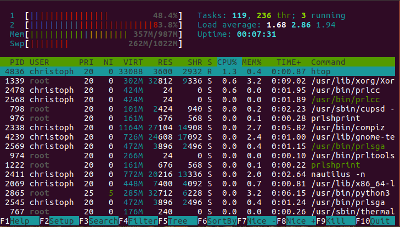
\includegraphics{images/htop.png}
\end{center}
\caption{ HTOP Upper interface will be the base for the CLI }
\label{HTOP}
\end{figure}

\begin{figure}
\begin{center}
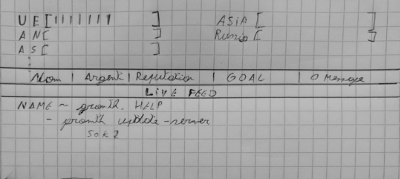
\includegraphics{images/CLITest.png}
\end{center}
\caption{ Drawing of the idea of the CLI }
\label{CLITest}
\end{figure}


%%% Local Variables: 
%%% mode: latex
%%% TeX-master: "cahierDesCharges"
%%% End: 